\documentclass[12pt,a4paper,oneside,english]{book}

\usepackage{cite}


%\usepackage[latin1]{inputenc}

%\usepackage[T1]{fontenc}
\usepackage[english]{babel}
\usepackage{amsmath}
\usepackage{amsfonts}
\usepackage{amssymb}
\usepackage{graphicx}
\usepackage{subfig}
\usepackage{fancyhdr}
\usepackage{appendix}
\usepackage{hyphenat}
\usepackage{pdfpages}
%\usepackage{tocloft} % For TOC customization ( table of contents )
\usepackage{array,multirow,makecell}
\newcolumntype{C}[1]{>{\arraybackslash}p{#1}}

\usepackage{enumitem}
\setlist{leftmargin=*,itemsep=0pt}

\usepackage{centernot}
\usepackage[linesnumbered,ruled,vlined,english,onelanguage]{algorithm2e}

\usepackage{quotchap}
\makeatletter
\renewcommand{\@makechapterhead}[1]{
 \chapterheadstartvskip
 {\size@chapter{\sectfont\raggedright
 {\chapnumfont
 \ifnum \c@secnumdepth >\m@ne
 \if@mainmatter\thechapter %frontmatter for roman numerals
 \fi\fi
 \par\nobreak}
 {\raggedright\advance\leftmargin10em\interlinepenalty\@M #1\par}}
 \nobreak\chapterheadendvskip}}
\makeatother
\renewcommand*{\chapterheadendvskip}{\vspace{2cm}}
%\renewcommand{\thechapter}{\Roman{chapter}} % Set chapter numbering to Roman numerals


\usepackage{geometry}
\geometry{hmargin=2cm,vmargin=2cm}

\pagestyle{fancyplain}
\lhead{\fancyplain{}{\nouppercase{\textit{\leftmark}}}}
\chead{\fancyplain{}{}}
\rhead{\fancyplain{}{}}
\lfoot{\fancyplain{}{}}
\cfoot{\fancyplain{}{}}
\rfoot{\fancyplain{\thepage}{\thepage}}
\renewcommand{\headrulewidth}{1pt}
\renewcommand{\footrulewidth}{1pt}

\renewcommand{\thesection}{\Roman{section}} % Set section numbering to Roman numerals % previously \arabic{section}

\usepackage{titlesec}
\titleformat{\paragraph}{\fontsize{11}{10}\bfseries}{\theparagraph}{1em}{}
\titlespacing*{\paragraph}{0pt}{10pt plus 2pt minus 0pt}{0pt plus 2pt minus 0pt}

\setcounter{secnumdepth}{4}
\setcounter{tocdepth}{4}

\usepackage{array}
\usepackage{multirow}
%\addto\captionsfrench{\def\tablename{\textsc{Tableau}}}

%\DefineBibliographyStrings{french}{urlseen = {},}

\setlength{\parskip}{0pt}%was 8 : space between paragraphs
\setlength{\parindent}{1.5em}%was 1.5 : indentation of paragraphs

\usepackage{setspace}

\usepackage{url}

\usepackage{hyperref}
% Comment before printing to remove links' colors
\definecolor{darkblue}{rgb}{0.0, 0.0, 0.5}
\hypersetup{
 colorlinks,
 linktocpage=true,
 linkcolor={darkblue},
 citecolor={darkblue},
 urlcolor={blue}}

\sloppy

\author{You}
\title{Internship Report}

\begin{document}
\pagenumbering{gobble}
\includepdf[pages=-]{FrontPage.pdf}
\chapter*{Acknowledgments}

\frontmatter %here yothhrou les num des pages en bas 
\chapter*{Abstract}
\normalsize{Write your abstract here.

\medskip
{\noindent \textbf{Keywords: ..., ... .} }

\spacing{1}
\tableofcontents{}
\newpage 
\listoffigures
\newpage 
\listoftables
\newpage
\spacing{1.4}
\chapter*{List of acronyms}
%\addcontentsline{toc}{chapter}{Liste des acronymes}
\markboth{List of acronyms}{}
\begin{itemize}
\item \textbf{Abbrev.} Abbreviation
\end{itemize}

\frontmatter %here yothhrou les num des pages fl contnent
%\frontmatter  %to have roman page numbering in the beginning
%\mtcaddchapter[Introduction g�n�rale]

\chapter*{Introduction}
\addcontentsline{toc}{chapter}{Introduction}
\markboth{Introduction}{}

\chapter{Company Presentation} % we should metion that there are a lot of spacing between title of chapter and sctions

\label{ch:1er}
\section{Overview}
Founded in 2020, and located in both Meudon la forêt , Meudonn France and tunis, Tunisia, 
Hydatis is dedicated to helping early-stage companies leverage the latest data intelligence and digital technologies to solve real-world challenges, becoming, since then, a leading technology startup studio with a proven track record.
\begin{figure}[h!] % placement options: h=here, t=top, b=bottom, p=page
    \centering
    
\includegraphics[width=0.2\textwidth]{images/hydatiss.png}
    \caption{Logo of Hydatis}
    \label{fig:hydatis}
\end{figure}

Hydatis specializes in AI, machine learning, blockchain, big data Analysis and more. Hydatis's team of technology experts is dedicated to building scalable and sustainable businesses, with a focus on creativity, strategy, and technology alongside with a vast network of partners and investors and a strong reputation in the technology industry.
\begin{figure}[h!] % placement options: h=here, t=top, b=bottom, p=page
    \centering
    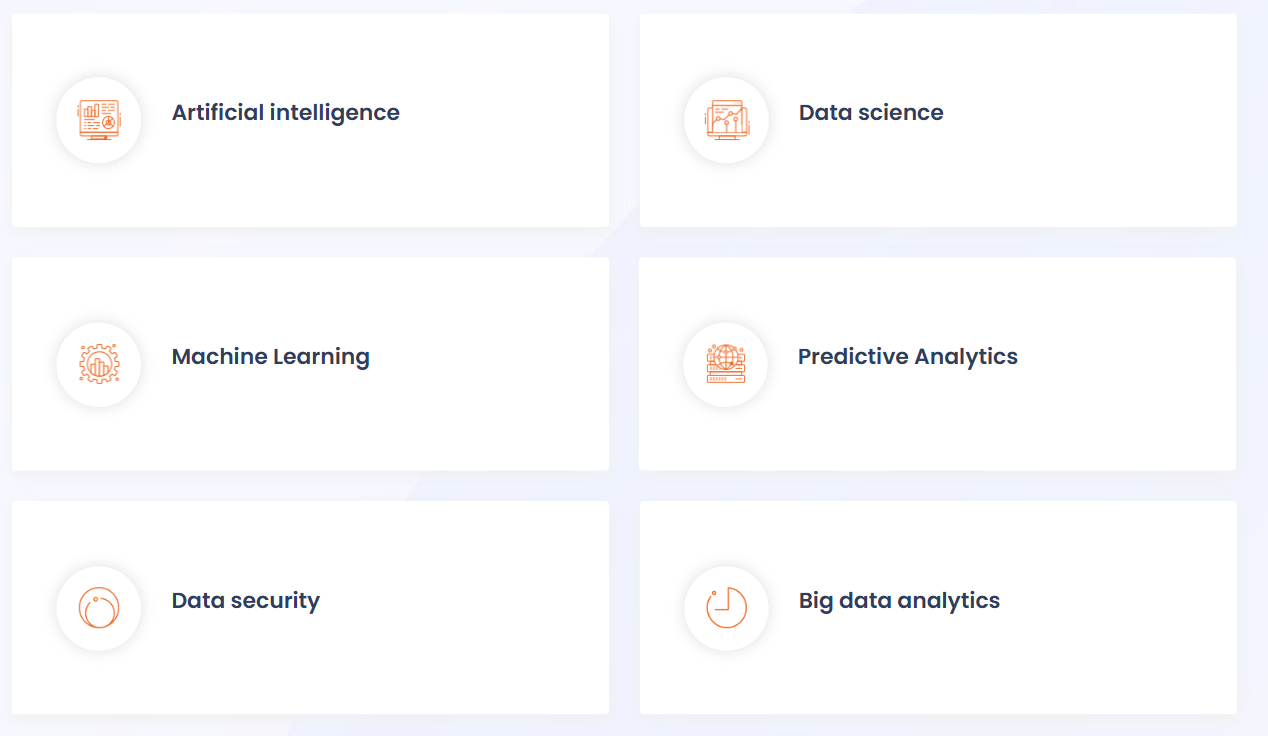
\includegraphics[width=0.699\textwidth]{images/Expertise_hydatis.png}
    \caption{Hydatis' Areas of Expertise}
    \label{fig:Expertise_hydatis}
\end{figure}

\section{Sectors of Activities}%and services offered
Hydatis is a product-focused Tech venture studio offering a range of services tailored to the unique needs of each startup, including:
 business planning, product development, marketing, and fundraising. 
%With their expertise in data analytics, machine learning, and other advanced technologies, 
Leveraging technology and entrepreneurship, they help clients turn data into actionable insights that drive business success.
%help businesses make big decisions about their future by making tangible versions of tomorrow.
\subsection{Services offered}
\begin{itemize}
    \item \textbf {Software development Services}
    \item \textbf{CTO as a service}
    \item \textbf{IT Consulting}
    \item \textbf{Devops Consulting}
    \item \textbf{and a lot more...}
\end{itemize}
\begin{figure}[h!]
    \centering
    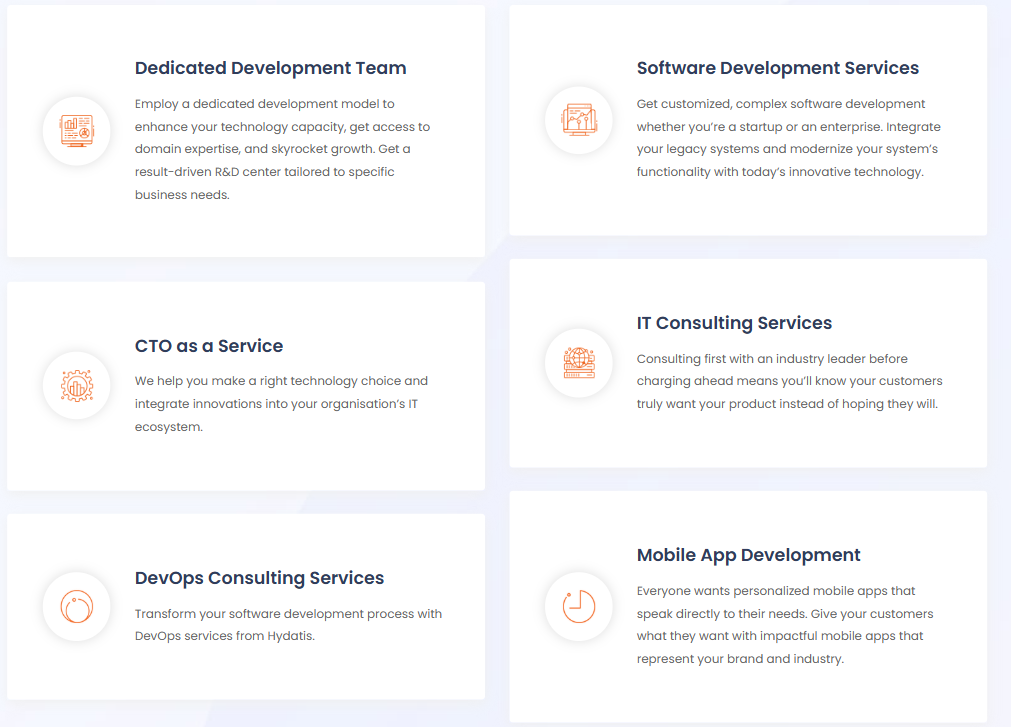
\includegraphics[width=0.9\textwidth]{images/services_hydatis.png}
    \caption{Hydatis' Services}
    \label{fig:Services_hydatis}
\end{figure}

\section{Organizational structure and Human Capital} % eithr this part will be deleted or the susection in the activities section will be modified and either discard items or having an individual subsection
Hydatis with a flat organizational structure that reflects its startup studio roots, led by  expertised directors who drive strategy and innovation alongside a talented crew of entrepreneurs and technologists, business strategists and network coordinators.

From AI specialists shaping cutting-edge products to strategists securing partnerships, and sicne its launch in 2020, these folks, with their varied backgrounds, suceeded to make Hydatis a powerhouse in the startup ecosystem.


\chapter{Internship Context and Objectives}
\label{ch:2eme}
\section{Problem Statement and Motivation} %Why
Crime is a major social problem in Tunisia, threatening public safety and disrupting the economy,ranging from theft to harassment, often leaving individuals vulnerable, especially at night or in isolated spots.
 
Traditional safety solutions such as manual reporting or basic wearable alarms have served as a foundational step in personal security. However they %struggle
suffer from critical limitations: 
The binary nature of a simple button press is usually unsufficient to distinguish between 
a genuine, life-threatening emergency,a false alarm, or a low-priority situation.
Additionally, the lack of contextual awarness results in inaccurate alerts and overwhelming emergency services with false positives. %Inaccuracy and Context Deficiency:
Giving the limited resources of emergency services (police, paramedics), false alarms divert critical attention away from genuine crises, incurring unnecessary costs and potentially delaying responses to real incidents. %Resource Depletion:


%The binary nature of a simple button press: unsufficient to distinguish between 
%a genuine, life-threatening emergency,a false alarm, or a low-priority situation. This leads to an unacceptably 
%high rate of false positives.

%  This gap hits home for Hydatis, the motivation behind this work is clear: we need to move beyond simple, reactive triggers
% and build smarter, faster ways to protect people by qualifying alerts with precision.
\subsection{Market Context and Existing Solutions}

Several commercial solutions exist in the personal safety market, including panic button apps like 
bSafe, location-sharing platforms like Life360, and wearable devices such as personal alarms. However,
 these solutions typically operate independently and lack the intelligent analysis needed to 
 differentiate between genuine emergencies and false alarms and ensure fast response to threats. 
 %, leading to the limitations described above.
Therefore, there is a clear need for an intelligent safety system that can analyze multiple data 
streams—location, audio, and behavioral patterns—to provide accurate, context-aware emergency 
detection while minimizing false positives.

%In State of the Art, you can include:
%Existing products (apps, devices, services → e.g., SOS apps, smartwatches with panic buttons, crime reporting platforms).
%Research/technical approaches (papers on anomaly detection, crime prediction models, wearable safety devices).
%Limitations of these (false positives, lack of contextual awareness, poor adoption, battery issues, limited reach, etc.).

%Detailed technical comparisons
%Algorithm discussions
%Academic literature reviews
%In-depth analysis of existing methods

%todo: reduce space in the footer ( especially see this page!)
%todo: and fama paget fihom khatt fl footer o whayed lee

\section{Description}% or scope : the "What." and "how" A high-level overview of the solution.

This project involves designing an AI-powered module for a Smart wearable Solution, aimed at enhancing personal safety through automated incident detection during my Summer internship at Hydatis.
The module integrates four key data streams: 
\begin{itemize}
    \item \textbf{Geospatial Analysis:} geospatial data derived from Tunisian crime datasets to identify high-risk areas.
    \item \textbf{Vocal Signal Processing:}  real-time vocal analysis to detect distress signals or key words such as calls for help.
    \item \textbf{Behavioral Profiling:} behavioral patterns to flag anomalies in user activitythat may indicate danger.
    \item \textbf{Decision Engine:} later, these components are fused into a cohesive system that processes and combines 
insights from each stream, offering a foundation for reliable alert qualification.
\end{itemize}
Though, detailed implementation will be explored in later sections.


\section{Core Mission, Objectives and Expected Results}

\subsection{Core Mission}
My core mission in this project is to develop an intelligent, multi-modal safety system that integrates  geospatial analysis, vocal processing, and behavioral profiling to transform personal security and  provide accurate , context-aware emergency detection that minimizes false alarms while ensuring genuine immediate attention to genuine threats  .

\subsection{Main Objectives}

\textbf{Technical Objectives:}
\begin{itemize}
    \item Achieve a minimum of 80\% accuracy in alert qualification.
    \item Minimize false positive rates. 
    \item Enable real-time processing  with response times under 5 seconds.
    \item Design a robust system capable of handling diverse scenarios and user behaviors.
\end{itemize}

\textbf{Implementation Objectives:}
\begin{itemize}

\item Process a Tunisian crime dataset for geospatial risk assessment.
\item Train a vocal ASR model adapted to Tunisian dialects for distress-related risk detection.
\item Prepare a vocal pipeline to analyse vocal patterns including: tone, rythm, and pitch.
\item Design a comprehensive database of processed behavioral patterns for every user.
   \item Integrate three distinct AI modules (geospatial, vocal, behavioral) into a cohesive system.
    \item Develop a proof-of-concept API for periodic risk assessment and scoring alerts.
    \item Ensure system scalability for potential deployment beyond Tunisia.
\end{itemize}

\subsection{Expected Results}
\begin{itemize}
\item A cleaned and structured Tunisian crime dataset inferred to geospatial risk analysis.
\item An ASR model integrated for vocal analysis in tunisian Arabic. %supporting real-time distress detection.
\item A vocal pipeline capable of analysing vocal patterns of stress and/or fear.
\item ML models designed for inferring  users behaviors.
\item A proof-of-concept multi-modal scoring system with sub-5-second responses.
\item APIs developed for periodic risk assessment and potential integration into a mobile or web interface.
\end{itemize}


\section{Internship timeline }% or planning %professionalism and project management skills.%%%%%often a Gantt chart)
%Timeline = just dates and deadlines
%Planning = timeline + methodology + resources + milestones

This project is structured over my two-month internship period at Hydatis, devided into:
\begin{itemize}
    \item \textbf{Weeks 1-2:} Initial research, dataset acquisition, and preprocessing.
    \item \textbf{Weeks 3-4:} Development of the geospatial analysis module and initial vocal processing pipeline.
    \item \textbf{Weeks 5-6:} Behavioral profiling model development and integration of the three AI modules.
    \item \textbf{Weeks 7-8:} Final system integration, testing, optimization, and documentation.
\end{itemize}

%todo: label the sections and subsections
%todo: diagramme de gantt!!!!

\chapter{Theoritical Foundations and State of the Art}
\label{ch:3eme}

% normalement we should put here:  State of the Art and Market Solutions section
% or subsection in the motivation and problem statement section: Existing Solutions and Limitations”
\section*{Introdunction}
This chapter presents the theoretical foundations underlying the multi-modal safety system developed in this project. 
The system integrates three distinct yet complementary technologies: geospatial analysis for location-based risk assessment, vocal signal processing for distress detection, and machine learning techniques for behavioral anomaly detection.
The first section examines GIS-based approaches to crime hotspot analysis and spatial pattern recognition, providing the foundation for our geospatial risk module. 
The second section explores density-based clustering algorithms, particularly DBSCAN and OPTICS, which form the core of our location risk assessment methodology. 
Finally, the third section reviews real-time geospatial risk assessment systems and their practical implementation challenges.
Together, these theoretical foundations establish the scientific basis for the integrated approach adopted in this project and position our 
work within the current state of research in intelligent safety systems.
%ghalt il faut revoir !
\section{Geospatical Analysis for Risk Prediction}
\label{sec:geospatial_theory}

%todo introooooo?? for chapter and sections too ?


\subsection{Anomaly Detection in Geographical Information Systems}
%create abstract GIS 
%the subsections will be discussed later
\subsection{Crime Hotspot Detection and Spatial Analysis}%or crime hotsport forecasting or the principe of crime hotspot analysis
% Geographic crime patterns, spatial autocorrelation, hotspot theory
%if we merge the  2 :
\subsection{GIS-Based Crime Hotspot Analysis and Spatial Patterns}


\subsection{Density-Based Clustering for Spatial Data}%or for geographic data
% DBSCAN and OPTICS algorithms, parameter selection, advantages for geographic data
\subsection{Real-time Risk Assessment Systems}%or relevance to risk prediction
% Current approaches, GPS-based risk scoring, challenges in real-time implementation




\section { Vocal Signal Processing for Distress Detection}
\section{Machine Learning for Behavioral Anomaly Detection}


\chapter{Design and implementation}
\label{ch:4eme}
\section{System Architecture and Data management}
\section{Implementation of the Geospatial Analysis Module}
\section{Implementation of the Vocal Signal Processing Pipeline}
\section{Implementation of the Behavioral Profiling Module} % or the Behavioral Anomaly Detection Module or the Machine Learning Module
\section{Final Decision Engine and System Integration}
%this may be merged with the first section (dont know shkoun shyemshi bahtha sahbou ( hawka naamlou referencing lel sections elli will tailor the details if nkaddmou el decision engine kbal les ai modules))

\chapter{Results and Discussion}

\section{Evaluation and Results}
\section{Discussion}








%\section*{Conclusion}
%\section{Conclusion}
\chapter*{Conclusion and perspectives}
\addcontentsline{toc}{chapter}{Conclusion and perspectives}
\markboth{Conclusion and perspectives}{}

\begin{appendix}
\chapter{Appendix 1}
Insert your appendixes here if you need.
\end{appendix}

%\spacing{1}
\bibliographystyle{unsrt}
\bibliography{references}
\end{document}